\begin{comment}
\title{parslTestbookQMCblog}
\author{Dr. Sou-Cheng Choi, Illinois Tech and SouLab, Joshua Jay Herman (QMC Development Team)}
\date{September 2025}

\maketitle
Accelerating QMCpy Notebook Tests with Parsl
\end{comment}

\subsection{Introduction}


 This blog provides a summary of the speedup of notebook regression testing presented in our talk at ParslFest [1] %, sponsored by Globus Compute, 
 and highlights the subsequent directions of the work. Regression testing of notebooks is massively parallel and resource-intensive.

\subsection{Methodology}
 Choosing Testbook \cite{} was primarily motivated by the usability of actually writing a test (one that would even execute the notebook itself). It also fits well with our tests in a separate directory, which we already have implemented other tests. of without requiring execution of the full notebooks for clarity. Then we made a test harness that we could also have Parsl [2] execute our testbook unittests since it is embarrassingly parallel.

\subsection{Results}
To determine a baseline speedup with a subset of notebooks we saw a  speedup. 
After increasing our test coverage, which expanded our work to look for syntax errors in more notebooks, 
we see now a 4x speedup which is consistent with our expectations. 

\begin{center}
%\begin{minipage}{0.7\textwidth}
    \centering
    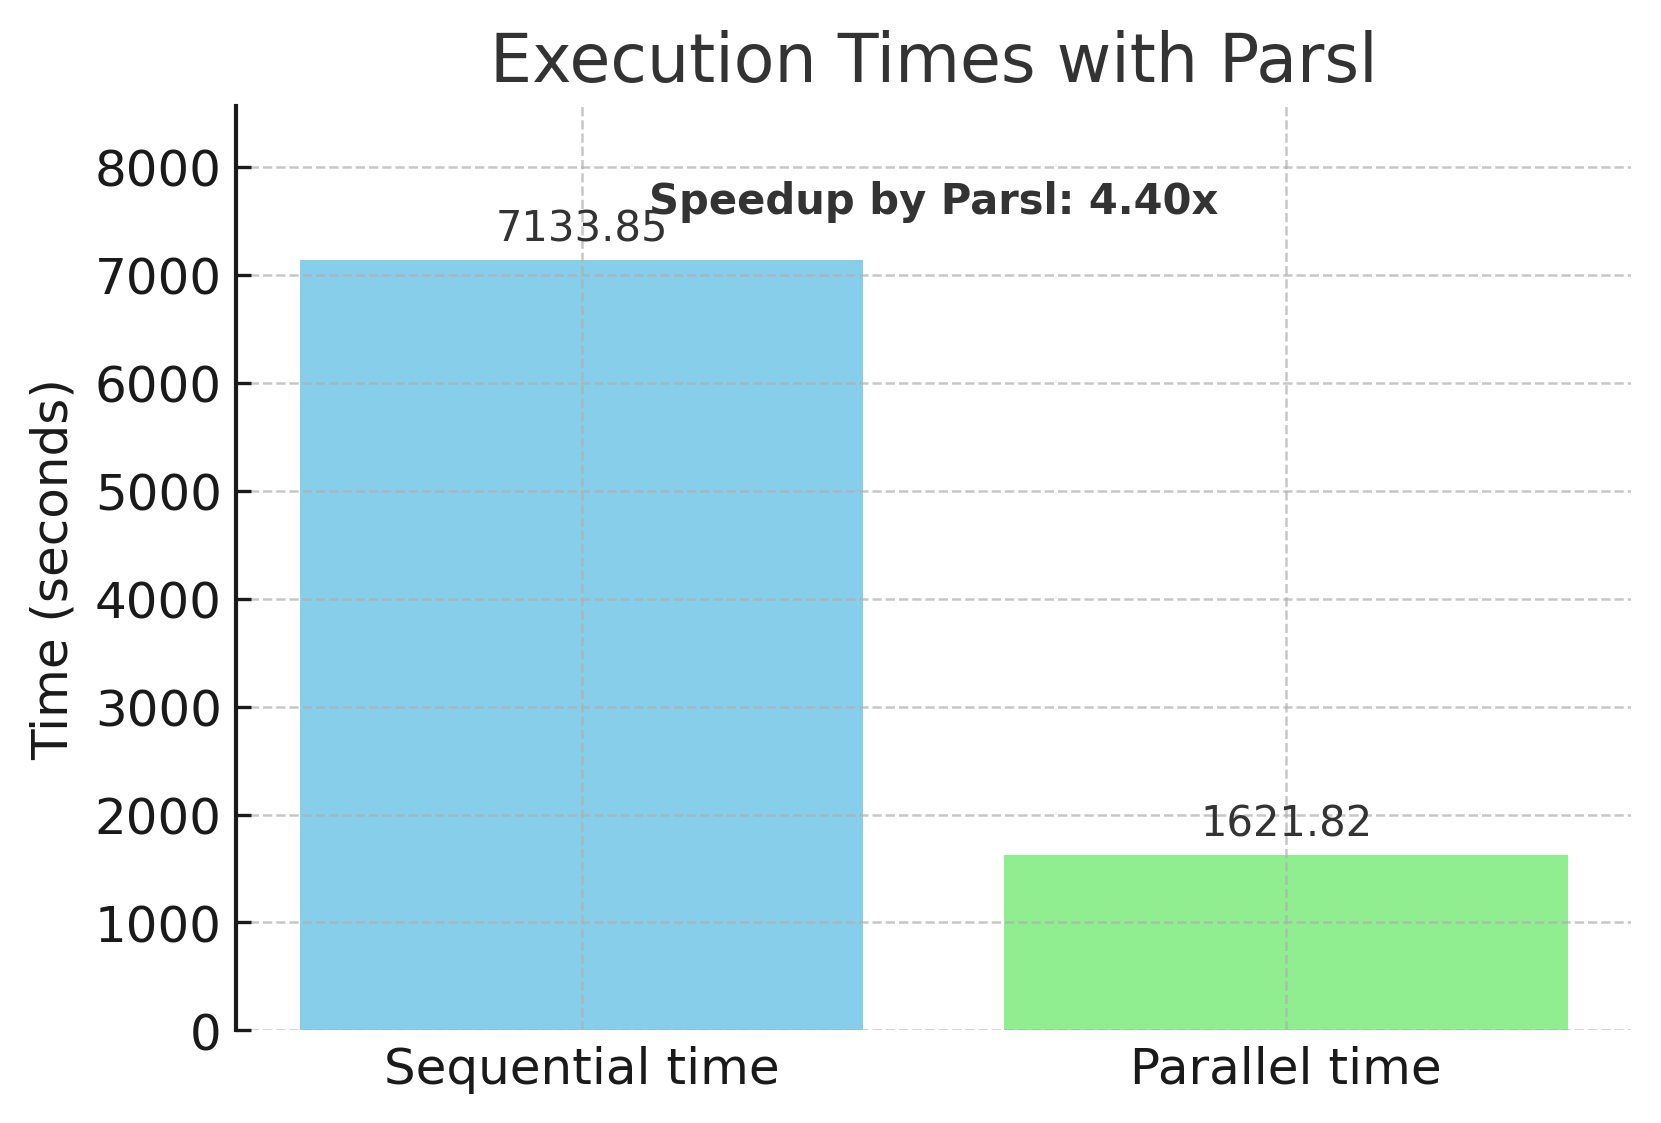
\includegraphics[width=.7\textwidth]{booktests/parsl_speedup_chart_no_x_lines.png}
    \captionof{figure}{Parallel testing speedup achieved using Parsl framework across varying numbers of processor cores}
    \label{fig:parsl_speedup}
%\end{minipage}
\end{center}

\subsection{Further Work}

Due to the above results, this points to the fact that we should extend our testing to doctest and pytests in Parsl.

Now, since many people have multi-core processors, we can make our individuals more productive so that our tests can show that no regressions have been introduced faster.

The last but not least of the feedback of the presentation of this work to the Parsl group would be that the system is very general. This implies that a distributed test system could be interesting for Parsl users to distribute their own test workloads. 
Also, extending our work to not just test Juypter notebooks but also Python based doctests, unit testing using pytest and or unitteSCsts and Cucumber tests for Behavior-Driven Development.


%TODO 
%Github actions? Done
%Put img here Done 
%Add refrences to parsl projects done
%work on wording suggestions.Done

\begin{thebibliography}{6}

\bibitem[1]{parslfest2025}
Parsl Project. 2025. Globus Compute + ParslFest 2025: Annual Community Gathering (Hybrid), August 28-29, University of Chicago. https://parsl-project.org/parslfest/parslfest2025.html

\bibitem[2]{parsl2019}
Yadu Babuji, Anna Woodard, Zhuozhao Li, Daniel S. Katz, Ben Clifford, Rohan Kumar, Luksaz Lacinski, Ryan Chard, Justin M. Wozniak, Ian Foster, Michael Wilde and Kyle Chard. Parsl: Pervasive Parallel Programming in Python." 28th ACM International Symposium on High-Performance Parallel and Distributed Computing (HPDC). 2019. 10.1145/3307681.3325400

\bibitem[3]{qmcpy2023}
Choi, S.-C. T., Hickernell, F. J., Jagadeeswaran, R., McCourt, M. J., \& Sorokin, A. G. (2020--2025).
QMCPy: A quasi-Monte Carlo Python Library (Version 2.1).
DOI: \url{https:/doi.org/10.5281/zenodo.16822646}. 
Retrieved from \url{https:/www.qmcpy.org}.



\end{thebibliography}
